% Seccion: Contexto del sistema
% Autor de la seccion: Jonathan Javier Rivera Suarez
% Version preliminar: entidades y flujos a validar con la entrevista.

\section{Contexto del sistema}
\label{sec:contexto}

El contexto de un sistema es la parte del entorno que es relevante para definir y entender sus requisitos; el límite del sistema separa lo que el sistema hace de lo que hacen las personas y sistemas externos con los que se comunica \cite{pohl2025}.

La Figura~\ref{fig:contexto} muestra el SGMC como un único proceso rodeado por las entidades externas. Cada flecha representa un flujo de datos con nombre; no se muestra cómo el SGMC procesa esos datos, porque eso corresponde a etapas posteriores. Su fuente editable es el archivo \texttt{diagrama\_contexto.puml} de la carpeta \texttt{modelos}.

\begin{figure}[htbp]
\centering
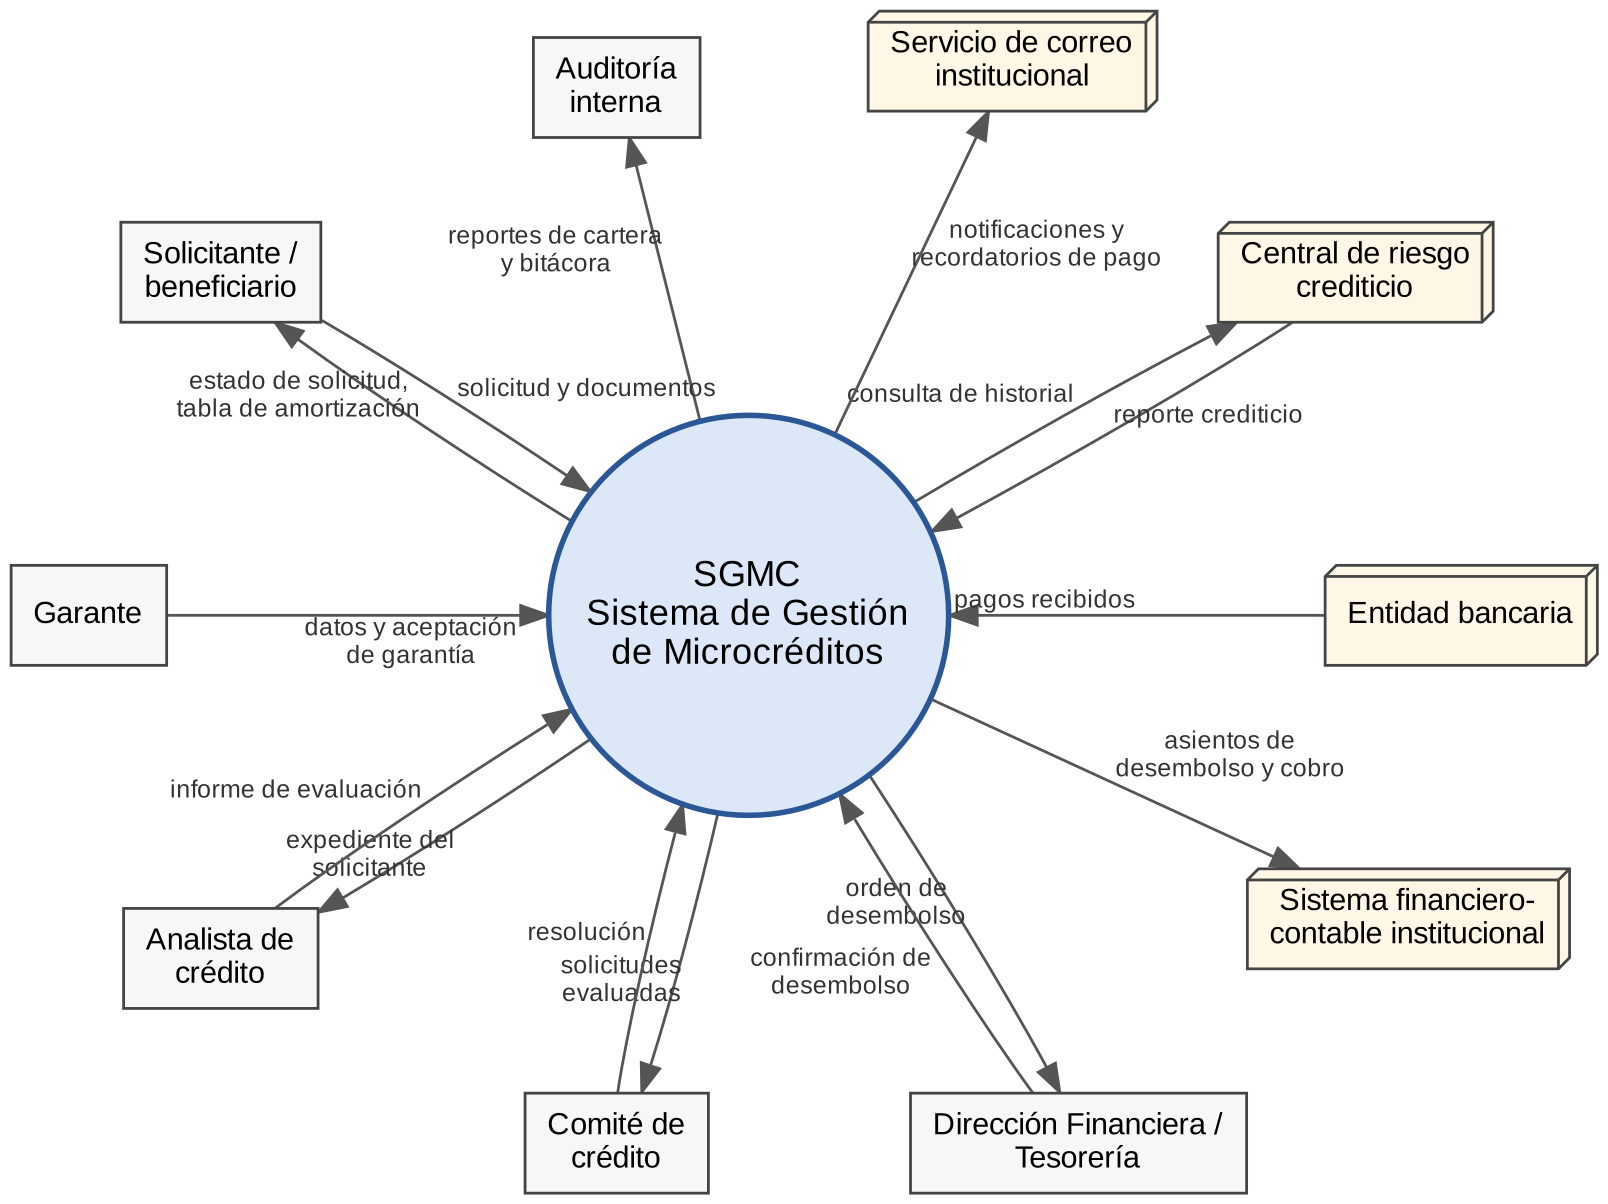
\includegraphics[width=\textwidth]{figuras/diagrama_contexto.png}
\caption{Diagrama de contexto del SGMC (versión preliminar).}
\label{fig:contexto}
\end{figure}

\subsection{Límite del sistema}

\textbf{Dentro del límite} queda lo que el SGMC realiza: registrar solicitudes y sus documentos, armar el expediente para el analista, registrar la resolución del comité, generar la orden de desembolso y la tabla de amortización, registrar los pagos, emitir notificaciones y producir reportes de cartera.

\textbf{Fuera del límite} quedan las decisiones y servicios de terceros: la aprobación de cada crédito (la toma el comité; el sistema solo la registra), la transferencia del dinero (la ejecuta la entidad bancaria), la contabilidad institucional, el cálculo del historial crediticio de la central de riesgo y el envío físico del correo.

La Tabla~\ref{tab:entidades} resume las entidades externas y los datos que intercambian con el sistema.

\begin{table}[htbp]
\centering
\caption{Entidades externas y flujos de datos del SGMC.}
\label{tab:entidades}
\small
\begin{tabularx}{\textwidth}{@{}>{\raggedright\arraybackslash}p{3.4cm}>{\raggedright\arraybackslash}X>{\raggedright\arraybackslash}X@{}}
\toprule
\textbf{Entidad externa} & \textbf{Envía al SGMC} & \textbf{Recibe del SGMC} \\
\midrule
Solicitante / beneficiario & Solicitud y documentos & Estado de la solicitud, tabla de amortización \\
Garante & Datos y aceptación de la garantía & --- \\
Analista de crédito & Informe de evaluación & Expediente del solicitante \\
Comité de crédito & Resolución (aprobada o negada) & Solicitudes evaluadas \\
Dirección Financiera / Tesorería & Confirmación de desembolso & Orden de desembolso \\
Auditoría interna & --- & Reportes de cartera y bitácora \\
Sistema financiero-contable & --- & Asientos de desembolso y cobro \\
Entidad bancaria & Registro de pagos recibidos & --- \\
Central de riesgo crediticio & Reporte crediticio & Consulta de historial \\
Servicio de correo institucional & --- & Notificaciones y recordatorios de pago \\
\bottomrule
\end{tabularx}
\end{table}

Dos entidades requieren confirmación con la organización: la central de riesgo, porque no se sabe si la institución consulta historiales externos, y la entidad bancaria, porque los pagos podrían recibirse también en ventanilla. Si alguna no aplica, se retirará del diagrama y de la tabla.


